\section{Parallel Space Solution of a nonlinear PDE using MPI}
\subsection{Domain decomposition}
%In your report, explain your chosen method of domain decomposition.
%Discuss why this method was selected and analyze its implications on the performance of the application.
%Consider aspects such as load balancing, communication overhead, and computational efficiency in your analysis.
The domain was decomposed using the non-periodic 2D Cartesian domain decomposition strategy, where the grid is divided into smaller rectangular subgrids, which are then assigned to a MPI processes. This method is suited for problems where you have grid and update the values on said grid with a stencil. Furthermore in our case the work is evenly distributed over the grid, which makes this method ideal, because it is simple and results in a good work balancing.
The topoloy created by the 2D Cartesian domain, also leads to efficient exchanging of neighboring ghost cells which reduces the communication overhead significantly.
Another plus point is that it is very scalable and can be easily used with varying number of processes.

% \subsection{Parallel I/O}

\subsection{Linear algebra kernels}
%Please briefly explain in your report which functions you modified and which you did not.
The primary rational used in order to decide which functions needed to be updated with MPI code was if the function needed to compute a result from distributed data across the processes or if the computation are done independently on each process. The two functions that modified were:
\begin{itemize}
	\item \texttt{hpc\_dot}: Added a \texttt{MPI\_Allreduce} in order to compute the global sum of the inner local product values.
	\item \texttt{hpc\_norm2}: Similar to the dot product the same MPI function was used to computed the global squared norm.
\end{itemize}
All the other functions can be used locally on the subdomain without needing to share the result, therefore no modification was needed.

\subsection{The diffusion stencil}
%Implement the ghost cell exchange between neighboring processes. See Fig. 1 for an illustration. Use non-blocking point-to-point communication with the objective to overlap computation and communication.
%Explain your approach in your report.
The non-blocking point-to-point MPI communication was used to exchange the ghost cells between processes. The non-blocking approach was used to overlap communication and therefore improve performance.
As the initial step the ghost buffers are filled with the boundary values from the local domain, corresponding to the direction they are sent. Furthermore the buffers for the receiving ghost cells are initialized.
Next the ghost are exchange using a non-blocking communication using \texttt{MPI\_Isend} and \texttt{MPI\_Irecv}, the order in which the send and received are executed does not matter due to the communication being non-blocking, but it is important that there is for each send there is a corresponding receive command. I decided to group them by direction as seen in Listing \ref{lst:operator}.
\begin{lstlisting}[language=C++, label=lst:operator, caption=Non-blocking send and receive pattern]
  // Send/recv east
  MPI_Isend(buffE.data(), buffE.xdim(), MPI_DOUBLE, domain.neighbour_east, 0,
            domain.comm_cart, &send_req[0]);
  MPI_Irecv(bndE.data(), bndE.xdim(), MPI_DOUBLE, domain.neighbour_east, 1,
            domain.comm_cart, &recv_req[1]);
  // Send/recv west
  MPI_Isend(buffW.data(), buffW.xdim(), MPI_DOUBLE, domain.neighbour_west, 1,
            domain.comm_cart, &send_req[1]);
  MPI_Irecv(bndW.data(), bndW.xdim(), MPI_DOUBLE, domain.neighbour_west, 0,
            domain.comm_cart, &recv_req[0]);

  // Send/recv north
  MPI_Isend(buffN.data(), buffN.xdim(), MPI_DOUBLE, domain.neighbour_north, 2,
            domain.comm_cart, &send_req[2]);
  MPI_Irecv(bndN.data(), bndN.xdim(), MPI_DOUBLE, domain.neighbour_north, 3,
            domain.comm_cart, &recv_req[3]);

  // Send/recv south
  MPI_Isend(buffS.data(), buffS.xdim(), MPI_DOUBLE, domain.neighbour_south, 3,
            domain.comm_cart, &send_req[3]);
  MPI_Irecv(bndS.data(), bndS.xdim(), MPI_DOUBLE, domain.neighbour_south, 2,
            domain.comm_cart, &recv_req[2]);
 
// the interior grid points
  for (int j = 1; j < jend; j++) {
    for (int i = 1; i < iend; i++) {
      f(i, j) = -(4. + alpha) * s_new(i, j)         // central point
                + s_new(i - 1, j) + s_new(i + 1, j) // east and west
                + s_new(i, j - 1) + s_new(i, j + 1) // north and south
                + alpha * s_old(i, j) +
                beta * s_new(i, j) * (1.0 - s_new(i, j));
    }
  }
  MPI_Waitall(4, recv_req, MPI_STATUSES_IGNORE);
\end{lstlisting}
The main reason why we use non-blocking communication is to overlap communication with computation, hence it is of upmost importance where the wait clause is placed. Because for computing the inner grid points the ghost cells are not necessary, we only need to ensure that all messages were received after the inner grid points calculation and before the boundary grid points are computed. In Listing \ref{lst:operator} the \texttt{MPI\_Waitall} for all the receiving requests is placed after the interior grid points for computed.
\subsection{Strong scaling}
The graphs seen in illustration \ref{fig:strong_scaling} show the strong scaling behavior of the mini application using MPI \ref{fig:mpi-strong} and OpenMP \ref{fig:openmp-strong} for its implementation. For both implementation were run on a single node on the Rosa cluster. Analyzing the MPI implementation we can clearly see that the execution time decreases for all grid sizes. Larger grid sizes benefit more from the parallelization, due to the computation outweighing the communication overhead. For smaller grid sizes on the other hand the reduction of execution flattens out when the communication overhead becomes large in relation to computation.\newline
Comparing this result to the restults from Project 3, we can observe that MPI achieves better across all resolutions, especially for larger grids size due to iths distributed memory model. OpenMP on the other hand struggles when the thead size increases, especially for smaller grids. Furthermore, by enabling overlapping communication with computation, the MPI version redues idle time and improves scaling, compared to the OpenMP, where the memory is shared and this lead to potential bottlenecks, especially for larger thread count.
In conclusion for small and medium grid sizes the OpenMP is more suited due to it performing very similar to the MPI version and it is a lot easier and quicker to implement. For large grid sizes on the other hand it is advised to take the time and implement the MPI version.
% How does your code scale for different resolutions?
% Interpret your results and compare them to the OpenMP implementation of Project 3 in your report.
\begin{figure}[H]
	\centering
	\begin{subfigure}{0.8\textwidth}
		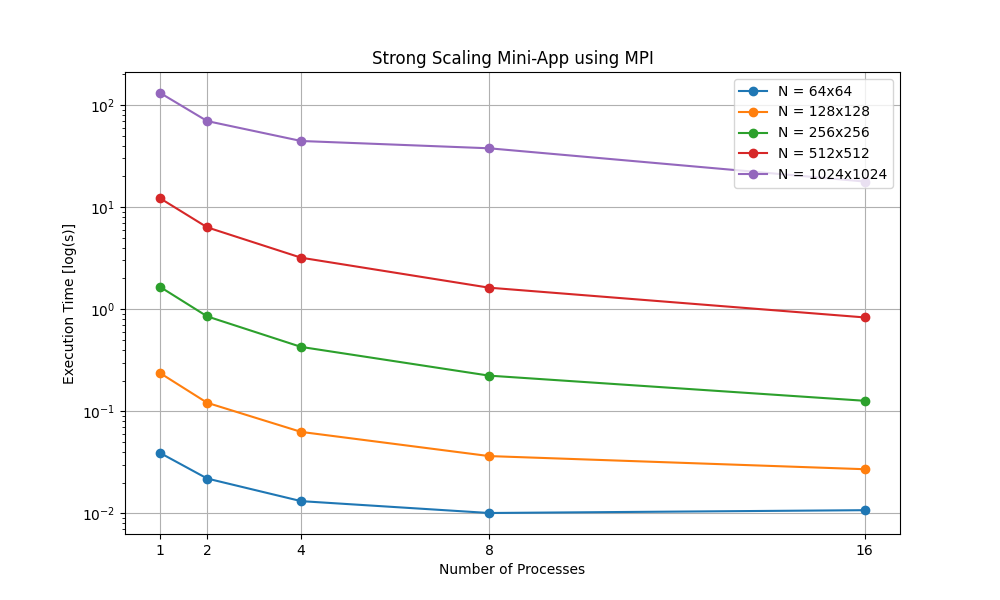
\includegraphics[width=\textwidth]{./media/strong_scaling.png}
		\caption{MPI}
		\label{fig:mpi-strong}
	\end{subfigure}
	\begin{subfigure}{0.8\textwidth}
		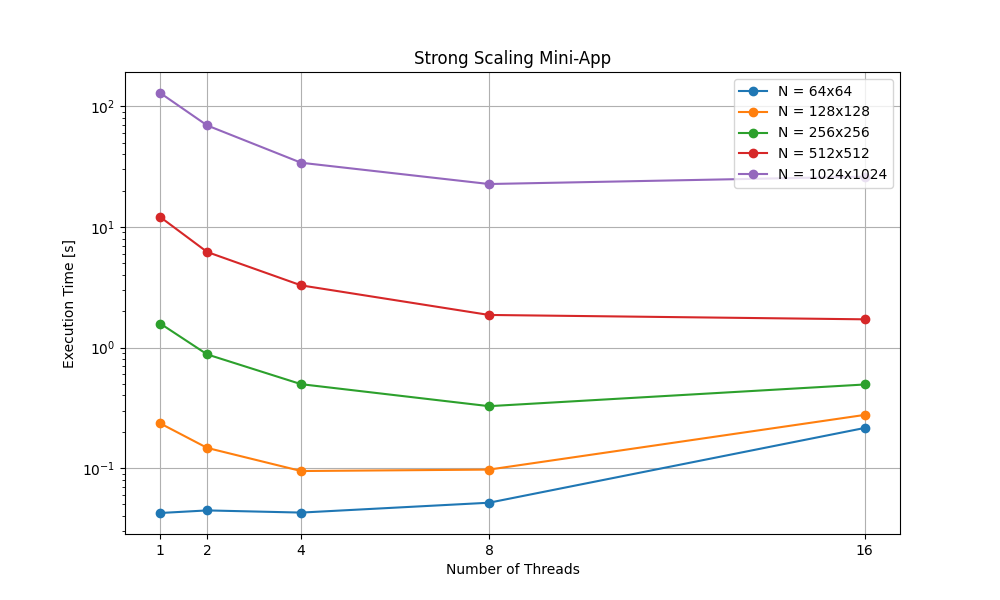
\includegraphics[width=\textwidth]{./media/strong_scaling_omp.png}
		\caption{OpenMP}
		\label{fig:openmp-strong}
	\end{subfigure}
	\caption{Strong Scaling}
	\label{fig:strong_scaling}
\end{figure}
\subsection{Weak scaling}
% How does code scale for constant work by process ratio?
% Interpret your results and compare them to the OpenMP implementation of Project 3 in your report.
The weak scaling of the mini-app for the MPI (\ref{fig:mpi-weak}) implementation, the efficiency decreases by a lot when increasing the base resolution, which is increased by multiplying the base resolution by the square root of the number processes. Larger base resolutions have stronger in increase of execution time compared to lower base resolution, this indicates inefficiencies as the problem size increases per process.
\newline
Comparing it to the result obtained in Project 3 for the OpenMP implementation, which can be seen in Subfigure \ref{fig:openmp-weak}. In terms of scaling efficiency the MPI outperforms the OpenMP version especially for larger problem sizes with higher number of processes. This shows that the MPI implementation handles large grid size more effectively, while the OpenMP's performance degrades.
One of the factor attested to that is the higher overhead usually encountered in application that use OpenMP. Eventhough the mini-app is rather inefficient, we can clearly see that the MPI version is closer to the optimal scaling indicated by the dashed lines. Overall the execution times are consistently lower for the MPI implementation. In conclusion MPI is the preferred choice especially if you have a larger workload, but it is also comes with the trade off of being more time intensive to implement.

\begin{figure}[H]
	\centering
	\begin{subfigure}{0.8\textwidth}
		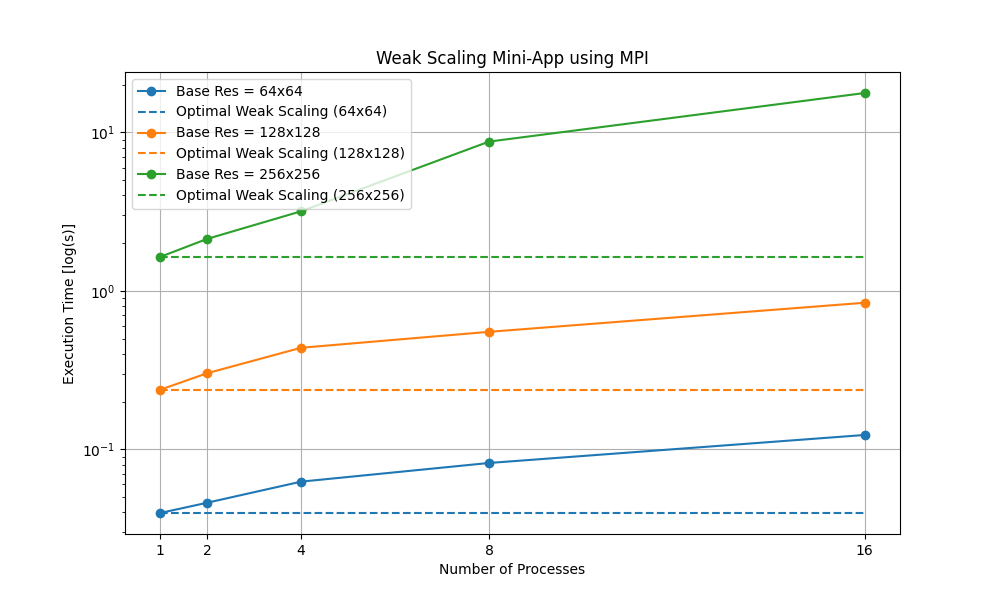
\includegraphics[width=\textwidth]{./media/weak_scaling.png}
		\caption{MPI}
		\label{fig:mpi-weak}
	\end{subfigure}
	\begin{subfigure}{0.8\textwidth}
		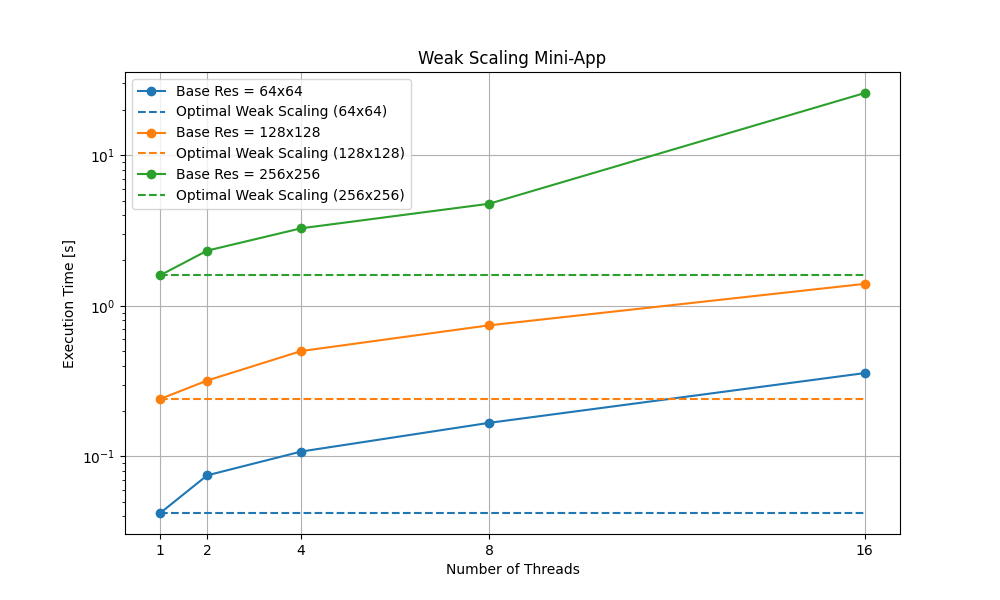
\includegraphics[width=\textwidth]{./media/weak_scaling_omp.png}
		\caption{OpenMP}
		\label{fig:openmp-weak}
	\end{subfigure}
	\caption{Weak Scaling}
	\label{fig:weak_scaling}
\end{figure}
